% \chapter{Introduction}
% \label{introduction}


% \begin{itemize}
    %     \item Chiral review \cite{epelbaum_frontiers}
    
    %     \item Weinberg \cite{WEINBERG1990}\\
    %         Weinberg \cite{WEINBERG1990} suggested using a most general Lagrangian
    %         satisfying spontaneously broken chiral symmetry and other symmetries and
    %         evolving pions together with low-energy nucleons.
    
    %         \item Epelbaum \cite{epelglockle98, epelglockle2000, epelglockle2003}
    %     \item The newest chiral force \cite{reinkrebs2018} 
    
    %     \item Arenhovel \cite{ArenhovelPhotodisint1991}
    %     \begin{itemize}
        %         \item He used different currents (`names, types')
        %         \item Approaches
        %     \end{itemize}
        % \end{itemize}
% \section{Historical overview}
        
% In the second half of XX century physical society faced
% a problem of describing low-energetic nuclear reactions.
% \gls{qcd} is hardly applicable here as it is nonperturbative 
% at low energies what complicates a lot search for the solutions \cite{Machleidt2011}. 


% \printglossary[type=\acronymtype]
% \printnoidxglossary[type=acronym]

\chapter{Introduction}

% \begin{itemize}
%     \item Why we study few nucleon systems
%     \begin{itemize}
%         \item Strong interactions (2N and 3N force investigation; QCD, relativistic effects)
%         \item Electro-magnetic processes (electrons-, photons-induced reactions) (Arenhovel did ...)
%         \item Weak interactions (neutrons)
%     \end{itemize}

%     \item Nuclear forces used in the thesis
%     \begin{itemize}
%         \item AV18
%         \item Chiral (scs, sms; difference between chiral models; regularization problem)
%     \end{itemize}

%     \item Currents used in the thesis (regularization of currents to be done)
    
%     \item Formalism \& numerical methods
%     \begin{itemize}
%         \item Lippman-Schwinger eq
%         \item Schrodinger eq for deuteron; wave functions (sms) for deuteron - figures, binding energy
%         \item Three body: Fadeev eq. for bound (He3, H3) and scattering states
%         \item Siegert theorem ?
%         \item Partial wave decomposition, states ($pq\alpha$), Jakobi momenta;
%         operators in PW decomp. (current); Mathematica for PW
%         \item Theoretical uncertainties: truncation error, cut-off dependency, chiral order dependency
%     \end{itemize}

%     \item Results (\textbf{find everything what I have calculated: all processes and energies} )
%     \begin{itemize}
%         \item H2 photodisintegration
%         \item He3 and H3 photodisintegration
%         \item Pion capture
%     \end{itemize}

%     \item Summary
    
%     \item References
% \end{itemize}

\subsection*{Why we study few nucleon systems}

The study of light nuclei and their reactions for the decades has been serving as an easiest way
to investigate particles in nuclei and forces between them. 
Convenient way to proceed may be to study an interaction of nucleus with
other nucleus, particles or electromagnetic probes
as electrons photons, muons, pions, neutrinos, hyperions etc. In most cases study of
 elastic or inelastic scattering is possible.
Whis can be done both theoretically or by 
performing relevant experiments to test if theory works.
People take into account that interactions may be caused by different forces
and therefore should be described in different ways. It can be
either strong, weak or electromagnetic interaction. It depends
on the type of particle being scattered and the target which reaction it is.

In past many experimental efforts have been undertaken and
electromagnetic reactions in light nuclei have been a point of interest for experimentalists for decades.
There are experimental data from the second half of XX century (e.g. \cite{Skopik1974}, \cite{Liuexp68}, \cite{Kose1969MeasurementsOT}, \cite{Kamae}) which is still 
useful when it comes to checking theory with results of measurements.    
There are a number of facilities providing a source of gamma rays (both low- and high-energetic)
and other particles which
have been operating over decades and still allow to perform experiments.
There are among other such groups and collaborations as TUNL \cite{TUNL}, MAMI \cite{MAMI}, 
NIKHEF \cite{NIKHEF}, HI$\gamma$S \cite{TONCHEV2005170} and others.
% In past many experimental efforts have been undertaken:
%   photon-induced breakup (see e.g. \cite{Skopik1974, rachek2007}),
% electro-disintegration (e.g. \cite{LAGET200549}), nucleon-deuteron scattering and other reactions
% have been studied. 
In order to describe the nuclear reactions properly many
components should be taken into account.
The most important are nucleon interations and nuclear current.
First of all, different forces may act on
the participants.


The strong nuclear force appear inside the nuclei and, among others, bound neutrons 
and protons together. The description of strong interactions is extremely
difficult as it deals not only with nucleon, but with their constituents: quarks
and gluons. \gls{qcd} is a modern theory
describing strong interactions, but, at the moment,
it is not applicable at low energies ($Q^2 \lesssim 1 GeV^2$).
In our situation various approaches are coming into the scene.
The most advanced are 
chiral effective theory, lattice calculation and others \cite{IOFFE2006232}, \cite{BEANElaticce}, \cite{Machleidt2011}.

Starting the study of three- (and more) nucleon systems it was found that 
strong 2N force is not enough to describe
the system and 3N force was introduced. The first applications of such
a force showed that it brings sufficient contribution and cannot be ignored \cite{GLOCKLE1982343}.
Contribution of the 3NF can be examined comparing binding energies of light nuclei calculated
with and without this part with respect to experimental values.  
For example, binding energy for $^3$H calculated with \gls{av18} potential
without 3NF gives $E_b(^3\mathrm{H}) = \SI{-7.628}{\mev}$ \cite{NoggaAV18}. There are different
models that might add a 3NF contribution to \gls{av18} (or other potential). 
Using the Tucson-Melbourne(TM) model \cite{Tucson-Melbourne}   results
in $E_b(^3\mathrm{H}) = \SI{-8.478}{\mev}$ and Urbana IX \cite{Urbana3NF} 3NF provide us with 
$E_b(^3\mathrm{H}) = \SI{-8.484}{\mev}$. 
Looking at the experimental value $E_b(^3\mathrm{H}) = \SI{-8.482}{\mev}$,
it is clear that 3NF contribution makes prediction much closer to the measurement.
The same situation is with other atoms: the 2NF binding energy for $^3$He (calculated with \gls{av18})
is $E_b(^3\mathrm{He}) = \SI{-6.917}{\mev}$, TM contribution makes it $E_b(^3\mathrm{He}) = \SI{-7.706}{\mev}$,
Urbana IX - $E_b(^3\mathrm{He}) = \SI{-7.739}{\mev}$, while experimental value
is $E_b(^3\mathrm{He}) = \SI{-7.718}{\mev}$.
Once more we can see the importance of 3NF contribution on the $\alpha$-particle's ($^4\mathrm{He}$) binding energy:
pure \gls{av18} gives $E_b(^4\mathrm{He}) = \SI{-24.25}{\mev}$, \gls{av18} + TN - \SI{-28.84}{\mev}, \gls{av18} + Urbana IX - \SI{-28.50}{\mev} and experimental value
is \SI{-28.30}{\mev}.

Whereas the first applications included only early simplified "realistic" 3N potential, the latter
investigations, based on more advanced models, only confirmed this statements \cite{StoksPhysRevC49, WIRINGAPhysRevC51}.
It was also used to construct four-nucleon (4N) bound state \cite{NoggaPhysRevLett}.

Electromagnetic force appears between charged particles like protons, electrons or pions.
Also, the force is transferred between charged particles and a photon, so 
in photon- and electron- scatterings on the nuclei an electromagnetic
force is necessary component of a description. Arenh\"{o}vel \cite{ArenhovelPhotodisint1991} 
studied electromagnetic process - deuteron photodisintegration,
applying different approaches and comparing the results with
experimental data.

The weak force...

...  

\subsection*{Models of strong interaction used in the thesis}

In order to model the nuclear potential, physicists often use phenomenological
or semi-phenomenological approaches. It allows them to combine
theoretical knowledge about processes and experimental data.

One of such models, which was used in current thesis is the Argonne V18 (AV18) \cite{AV18Wiringa}.
In order to construct NN force, authors combine
% analytical electromagnetic and 
one-pion-exchange parts
with phenomenological one and supplement them by electromagnetic corrections.
Free parameters were fitted to
the Nijmegen partial-wave analysis of $pp$ and $np$ data \cite{NijmegenPhysRevC.48.792}. 
Authors showed, that AV18 potential delivers good results
in the description of nucleon scattering data ($\chi ^2/data = 1.08$ for around \num{4000} $pp$ and $np$ scattering datasets) 
as well as deuteron properties (estimated binding energy is \SI{2.2247(35)}{\mev} vs experimental \SI{ 2.224 575(9)}{\mev}).


In the early 1990-ies Weinberg \cite{WEINBERG1990,WEINBERG1991} introduced 
an idea of using the most general Lagrangian
satisfying assumed symmetry principles and in particular
spontaneously broken chiral symmetry to 
describe nuclear interactions at low energies.
This idea together with \gls{eft} of \gls{qcd} 
led to the development of the \gls{ceft}
% a Chiral effective field theory ($\chi$EFT)
which nowadays has become one of the most advanced approach to
low-energy nuclear physics. While in \gls{ceft} it is possible to study processesor bound states directly,
it is also possible to describe nuclear potential, which can be next used in quantum equations,
e.g. Schr\"odinger equation.
 
For the \gls{eft} it is very important to 
define a quantity, which powers will determine a perturbation order.
In the \gls{ceft} there are two natural scales: so-called soft scale $Q \sim M_\pi$  -
the mass of pion and the hard scale -
$\Lambda_\chi \sim \SI{0.7}{\gev}$ - chiral symmetry breaking scale.
The ratio between these two scales $Q/\Lambda_\chi$
is being used as an expansion parameter in  \gls{ceft} with power
$\nu$: $\left(Q/\Lambda_\chi\right)^\nu$.
\footnote{Note that excat values of some parameters are still under discussion \cite{Epelbaum2004}. We follow here approach described by E.Epelbaum and collaborators, see e.g. \cite{reinkrebs2018}}

Possibility of deriving nuclear potential is an important feature of \gls{ceft}.
The potential, as occurs in an Lagrangian, is a perturbation expression of the same parameter $Q/\Lambda_\chi$.
Considering so-called irreducible diagrams (which cannot be split
by cutting nucleon lines), Weinberg \cite{WEINBERG1990,WEINBERG1991}
came to the expression for the powers $\nu_W$ of such diagrams

\begin{equation}
    \nu_W = 4 - A - 2C + 2L + \sum_i \Delta_i,
    \label{powers}
\end{equation}
where $i$ specifies a vertex number and

\begin{equation}
    \Delta_i \equiv d_i + \frac{n_i}{2} - 2.
    \label{Delta}
\end{equation}

In \eq{powers}, $C$ is a number of pieces which are connected, $L$ - the number of loops in the graph
and $A$ is a number of nucleons in the diagram.
In \eq{Delta}, $n_i$ is a number of nucleon field operators, $d_i$ - the number of insertions
(or derivatives) of  $M_\pi$.

The further analysis of \eq{powers} revealed some problems which occur 
for particular values of parameters in the equation, namely negative values of $\nu_W$ 
are possible while the order has to take integer values from 0 to infinity.
In order to deal with that, \eq{powers} 
was slightly modified adding $3A - 6$ to it  \cite{Machleidt2011, EPELBAUM2006_PROGRESS}:

\begin{equation}
    \nu = \nu_W + 3A  - 6 = -2 + 2A - 2C + 2L + \sum_i \Delta_i
    \label{powers_corrected}
\end{equation}


In \gls{ceft} the first order, "leading order" (LO, $\nu=0$) is followed 
by next-to-leading order (NLO, $\nu=2$)
\footnote{The $\nu=1$ order is completely vanished due to parity and time-reversal invariance,
so next-to-leading order stands for the second order of expansion.},
 next-to-next-to-leading order (N$^2$LO, $\nu=3$) and so on.
 At each chiral order, new interaction diagrams complete the potential.
 At LO there is a diagram which consists of 2 contact terms and the diagram
 implying one-pion exchange. Both diagrams reflect only 2NF as well
 as diagrams at NLO, where more contact terms are introduced together with two-pion 
 exchange topologies. Each subsequent order includes more and more sophisticated diagrams
 describing nucleons interaction
 via multiple  pion exchanges and various contact verteces.
 3NF appears at N$^2$LO while 4NF contributions are occuring at N$^3$LO.
 This establishes for the first time a systematic
way to include all the forces from the simplest diagrams at LO and gradually
adding more and more terms. 
It is also beneficial in the way that 
one can obtain results using chiral potential at different
orders and track which one gives larger or smaller contribution to the final prediction.
The highest order for which there is a derived term in potential
is N$^4$LO at the moment. Nevertheless leading F-wave contact interactions from N$^5$LO are included in the N$^4$LO+ potential,
which is currently regarded as a best possible potential within the model.
The progression of the chiral orders is reflected in a $\chi^2/datum$.
Leading order has only $\chi^2/datum = 73$ (with neutron-proton data with $E_lab = 0-100 \unit{\mev}$).
Each subsequent order has better and better results: NLO has $\chi^2/datum = 2.2$, N$^2$LO - $\chi^2/datum = 2.2$
and the final N$^4$LO+ has $\chi^2/datum = 1.08$ \cite{reinkrebs2018}.
Similar progression is observed for larger energies, e.g for $E_lab = 0-300 \unit{\mev}$)
$\chi^2/datum$ is 75, 14, 4.2, 2.01, 1.16 and 1.06 at LO, NLO, N$^2$LO, N$^3$LO, N$^4$LO and N$^4$LO+ respectively.
The proton-proton data description has similar trend, so $\chi^2/datum$ is 1380, 91, 41, 3.43, 1.67, 1.00 
for the same energy bin and chiral orders. At N$^4$LO+ $\chi^2/datum$ for proton-proton data
stands similar value (close to 1) as for neutron-proton, but the convergence comes a bit later and 
leading order has way worse description.
In my work I will use chiral potentials from LO to N$^4$LO+.

\begin{figure}[h]
    \begin{center}
    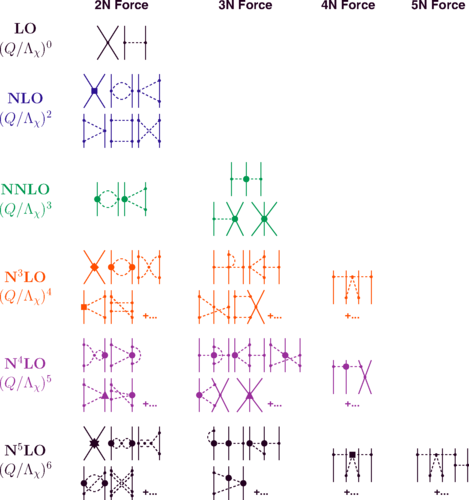
\includegraphics[width=0.6\textwidth]{Figures/chiral.png}
    \end{center}
    \caption{\tmp{get quality figure from \cite{Entem2017}}}
    \label{proton_rad}
\end{figure}

The general scheme outlined above was developed mainly by the Bochum-Bonn and Moscow-Idaho groups.
Both groups have similar approaches and were independently and almost simultaneously
developing own chiral potentials. In 1998 Epelbaum and colleagues from Bochum-Bonn group 
presented a first version of their chiral potential \cite{EPELBAOUM1998107, epelbaum2000two}.
Developing a more and more sophisticated versions with higher chiral orders, authors presented
N$^3$LO potential in 2005 \cite{epelbaum2005two} resulting with most advanced chiral potential at the moment - 
N$^4$LO+ \cite{reinkrebs2018}.
On the other side of the planet, in Idaho, the group from Moscow was also developing 
a chiral potential. Teir results from 2003 \cite{Entem2003}, following with later investigations \cite{Machleidt2005, Machleidt2010, Entem2017}.

There are a number of another approaches within \gls{ceft} utilized.
The group of Piarulli is using quite similar approach, including
the same chiral potentials with minor differences \cite{Piarulli2012,Piarulli2015}.

{\color{red} Machleidt, Ekstr\"om, pion-less EFT, Lattice EFT(Mesissner), Girlanda, Piarulli}


Technically the chiral potential may be derived both in coordinate and momentum spaces.
Nevertheless in both cases it requires regularizationcuts 
low coordinate values in order to avoid infinities 
(or high momentum values - in momentum space). 
The \gls{sms} potential is being regularized in its pion propagators
in the momentum space using the Gaussian form factor
$F(\vec{l}^2)$:

\begin{equation}
    F(\vec{l}^2) = e^{-\frac{\vec{l}^2 + M_\pi^2}{\Lambda^2}},
    \label{regulator}
\end{equation}
where $M_\pi$ is an effective pion mass and $\Lambda$ - is a cutoff parameter.

The form factor from \eq{regulator}, being used together with Feynman propagator,
ensures that long-range part of the forces has no singularities. 

The value at which
the cut is applied (cut-off value) is not fixed and usually calculations
are being performed for different cut-off values. The comparison
of such results may reveal stronger or weaker dependance and in perfect
case one will come up with such a potential, were the cut will
not affect results much. In \fig{potential_cutoff} 
I show values of the 2N potential $\matrixel{\vec{p}}{V}{\pvec{p}}$
as a function on the momentum $|\vec{p}|$ with fixed value $|\pvec{p}|$=0.054[fm].



\begin{figure}[htb]
    \begin{center}
    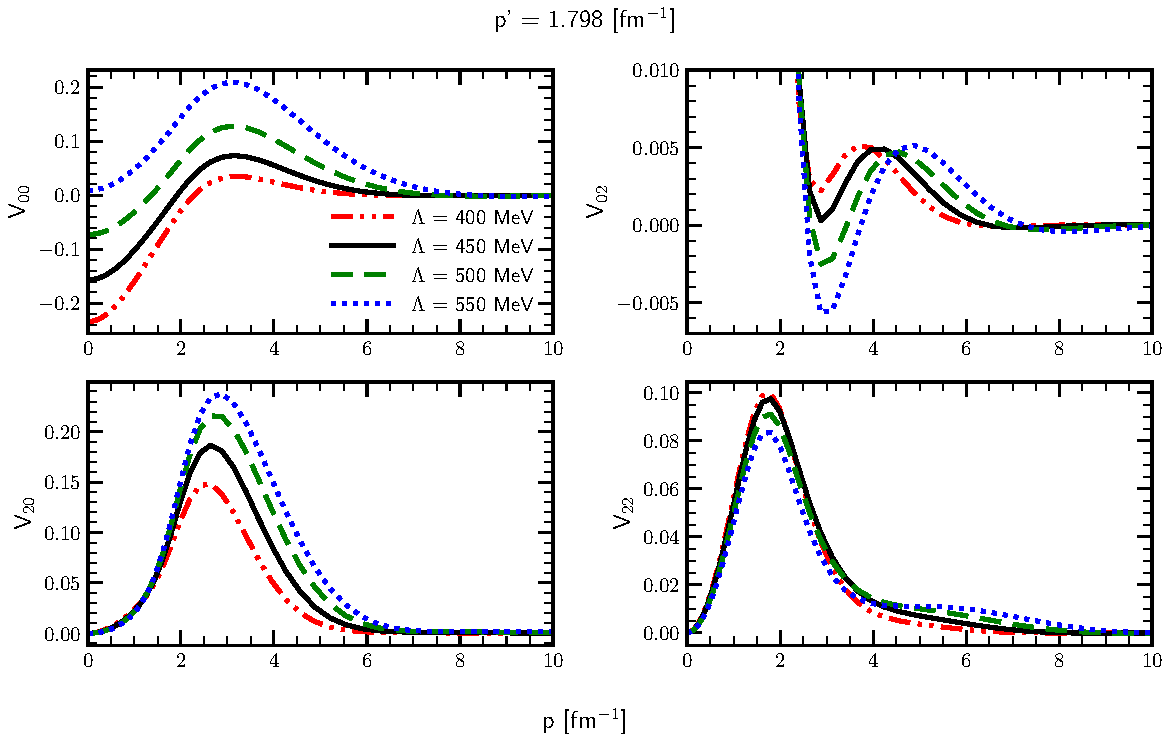
\includegraphics[width=0.95\textwidth]{PlotData/Deuteron/WAVEFUNC/potential_pp1.798.pdf}
    \end{center}
    \caption{Potential components as a function on the momentum $p$ with fixed
    value of the momentum $p'$=1.798 [fm?].
    }
    \label{potential_cutoff}
\end{figure}



The potential may be transformed from coordinate to momentum space (or vice versa),
but it is important at which frame the regularization was performed
and what was a regularization function. That's why there are different 
versions of chiral potential. One is \gls{scs} potential \cite{Epelbaum2014SCS}
and another one is similar, but with regularization applied in momentum space (\gls{sms} potential) \cite{reinkrebs2018}.


\subsection*{Currents}
 
% When it comes to the study of scattering processes on nuclei one has 
% to construct nuclear matrix elements, the crucial part 
% of which is nuclear current. The currents should be consistent with
% the force used

